\section{Giới thiệu về máy ảnh}

Máy ảnh (không làm thay đổi tính chất kỹ thuật, sau đây sử dụng từ "máy ảnh" để thay thế) là một thiết bị cơ bản trong thị giác máy tính, đóng vai trò thu thập dữ liệu hình ảnh từ thế giới thực. Để có thể sử dụng hình ảnh này cho các tác vụ phân tích và tái tạo 3D, chúng ta cần hiểu rõ về các đặc tính và mô hình của máy ảnh. Các đặc tính này thường được chia thành hai nhóm chính: tham số nội tại (gọi là  intrinsic) và tham số ngoài (gọi là extrinsic).

\subsection{Mô hình máy ảnh pinhole}
\label{subsec:pinhole_máy ảnh}

Mô hình máy ảnh pinhole là một mô hình hình học lý tưởng hóa, đơn giản nhất để mô tả quá trình tạo ảnh của một máy ảnh. Mặc dù bỏ qua các hiệu ứng quang học phức tạp của thấu kính thật (như méo ảnh, độ sâu trường ảnh), mô hình này lại là nền tảng toán học cốt lõi cho hầu hết các thuật toán trong thị giác máy tính và phục dựng 3D. Nó cung cấp một mối quan hệ hình học rõ ràng giữa các điểm 3D trong không gian và hình chiếu 2D của chúng trên mặt phẳng ảnh.

Các thành phần chính của mô hình máy ảnh pinhole bao gồm (xem Hình \ref{fig:pinhole_model}):
\begin{itemize}
    \item \textbf{Tâm quang học (Optical Center) hay Tâm chiếu (Center of Projection), $\vect{O}$}: Điểm duy nhất trong không gian mà tất cả các tia sáng từ vật thể đi qua trước khi tạo thành ảnh. Nó tương ứng với "pinhole" lý tưởng.
    \item \textbf{Mặt phẳng ảnh (Image Plane)}: Một mặt phẳng đặt vuông góc với trục quang học và cách tâm quang học $\vect{O}$ một khoảng bằng tiêu cự $f$. Đây là nơi hình ảnh của cảnh được hình thành. Trong máy ảnh thực tế, đây chính là bề mặt của cảm biến ảnh (sensor).
    \item \textbf{Trục quang học (Principal Axis)}: Đường thẳng đi qua tâm quang học $\vect{O}$ và vuông góc với mặt phẳng ảnh.
    \item \textbf{Điểm chính (Principal Point), $\vect{c}$}: Giao điểm của trục quang học với mặt phẳng ảnh. Trong mô hình lý tưởng, nó thường được giả định là nằm ở tâm của mặt phẳng ảnh/cảm biến.
    \item \textbf{Tiêu cự (Focal Length), $f$}: Khoảng cách từ tâm quang học $\vect{O}$ đến mặt phẳng ảnh dọc theo trục quang học.
\end{itemize}

\subsubsection{Phép chiếu phối cảnh (Perspective Projection)}

Trong mô hình máy ảnh pinhole, một điểm 3D $\vect{X}$ trong không gian được chiếu lên mặt phẳng ảnh thành một điểm ảnh 2D $\vect{x}'$ thông qua một phép chiếu gọi là **phép chiếu phối cảnh (perspective projection)**. Phép chiếu này tuân theo nguyên tắc đường thẳng: hình chiếu $\vect{x}'$ là giao điểm của tia sáng đi từ $\vect{X}$ qua tâm quang học $\vect{O}$ với mặt phẳng ảnh.

Do tia sáng đi qua tâm quang học, hình ảnh được tạo ra trên mặt phẳng ảnh đặt phía sau $\vect{O}$ sẽ bị lộn ngược (cả chiều trên-dưới và trái-phải) so với vật thể thực. Để thuận tiện cho việc phân tích toán học, người ta thường xem xét một **mặt phẳng ảnh ảo (virtual image plane)** đặt ở phía trước tâm quang học $\vect{O}$, cũng cách $\vect{O}$ một khoảng $f$ và song song với mặt phẳng ảnh thực. Hình chiếu $\vect{x}$ trên mặt phẳng ảnh ảo này sẽ cùng chiều và không bị lật so với vật thể (Hình \ref{fig:pinhole_model}). Các phân tích hình học sau đây thường dựa trên mặt phẳng ảnh ảo này.

% --- Hình ảnh minh họa ---
\begin{figure}[H] % [H] để ép ảnh hiển thị ngay tại vị trí code (cần gói float)
    \centering
    \begin{tikzpicture}[scale=0.9, >=stealth]
        % Hệ tọa độ máy ảnh (Xc, Yc, Zc)
        \coordinate (O) at (0,0); % Tâm quang học
        \draw[->, thick] (O) -- (4,0) node[below left] {$Z_c$}; % Trục Zc (trục quang học)
        \draw[->, thick] (O) -- (0,2.5) node[right] {$Y_c$}; % Trục Yc
        \draw[->, thick] (O) -- (-1.5,-1) node[below] {$X_c$}; % Trục Xc
        \fill (O) circle (1.5pt) node[below left] {$\vect{O}$};

        % Mặt phẳng ảnh ảo (tại Z=f)
        \def\focal{2} % Tiêu cự f
        \coordinate (c) at (\focal, 0); % Điểm chính
        \fill (c) circle (1pt) node[below] {$\vect{c}$};
        \draw[dashed, blue] (\focal, -1.5*1.2) -- (\focal, 1.5*1.2); % Đường trục y ảnh
        \draw[dashed, blue] (\focal-0.6*1.2, -0.4*1.2) -- (\focal+0.6*1.2, 0.4*1.2); % Đường trục x ảnh (xiên)
        \node[blue, above right] at (\focal+0.6*1.2, 0.4*1.2) {Image Plane ($\pi$)};
        \draw[<->] (O) -- (c) node[midway, above] {$f$};

        % Điểm 3D trong hệ tọa độ máy ảnh Xc
        \coordinate (Xc) at (3.5, 1.5);
        \coordinate (Xc_proj_xy) at (3.5, 0);
        \coordinate (Xc_proj_xz) at (3.5, 0, 1.5); % Giả định tọa độ x (chiều sâu khác)
        \fill (Xc) circle (1.5pt) node[above right] {$\vect{X}_c=(X_c, Y_c, Z_c)$};
        \draw[dotted] (Xc) -- (Xc_proj_xy);
        \node[right] at (Xc_proj_xy) {$Z_c$};
        \draw[dotted] (Xc) -- (0, 1.5);
        \node[above] at (0, 1.5) {$Y_c$};
        % Vẽ thêm chiếu lên mặt XZ nếu cần

        % Tia chiếu từ Xc qua O
        \draw[red, thick] (Xc) -- (O);

        % Giao điểm với mặt phẳng ảnh ảo (x)
        \path[name path=ray] (Xc) -- (O);
        \path[name path=image_plane] (\focal, -2) -- (\focal, 2); % Đường dài hơn để chắc chắn cắt
        \path[name intersections={of=ray and image_plane, by=x_proj}];
        \fill[red] (x_proj) circle (1.5pt) node[below right, red] {$\vect{x}=(x,y)$};
        \draw[dotted] (x_proj) -- (c); % Chiếu xuống trục Zc
        \draw[dotted] (x_proj) -- (\focal, 1.5*\focal/3.5); % Chiếu ngang sang trục Y ảnh ảo

        % Tam giác đồng dạng
        \draw[gray] (O) -- (Xc) -- (3.5, 0) -- cycle;
        \draw[gray] (O) -- (x_proj) -- (\focal, 0) -- cycle;
        \node[gray] at (1, 0.2) {$\triangle O Y_c Z_c$};
        \node[gray] at (2.5, 0.6) {$\sim$};
        \node[gray] at (3.2, 0.2) {$\triangle O y f$};

    \end{tikzpicture}
    \caption{Mô hình hình học của máy ảnh pinhole. Điểm 3D $\vect{X}_c$ trong hệ tọa độ máy ảnh được chiếu qua tâm quang học $\vect{O}$ lên mặt phẳng ảnh ảo tại điểm $\vect{x}$. Mối quan hệ giữa tọa độ 3D và tọa độ ảnh 2D được xác định bởi các tam giác đồng dạng.}
    \label{fig:pinhole_model}
\end{figure}
% --- Kết thúc Hình ảnh ---

\subsubsection{Mô hình toán học}

Xét hệ tọa độ máy ảnh với gốc tại tâm quang học $\vect{O}$, trục $Z_c$ trùng với trục quang học và hướng về phía cảnh, trục $X_c$ và $Y_c$ tạo thành hệ tọa độ thuận và song song với các trục $x, y$ của mặt phẳng ảnh. Mặt phẳng ảnh ảo nằm tại $Z_c = f$.

Một điểm $\vect{X}_c = [X_c, Y_c, Z_c]^T$ trong hệ tọa độ máy ảnh sẽ được chiếu lên mặt phẳng ảnh ảo thành điểm $\vect{x} = [x, y]^T$. Dựa vào nguyên lý tam giác đồng dạng (như minh họa trên Hình \ref{fig:pinhole_model}), ta có mối quan hệ:
\begin{equation} \label{eq:pinhole_projection}
\frac{x}{f} = \frac{X_c}{Z_c} \quad \implies \quad x = f \frac{X_c}{Z_c}
\end{equation}
\begin{equation} \label{eq:pinhole_projection_y}
\frac{y}{f} = \frac{Y_c}{Z_c} \quad \implies \quad y = f \frac{Y_c}{Z_c}
\end{equation}
Đây là các phương trình chiếu phối cảnh cơ bản của mô hình máy ảnh pinhole. Chúng cho thấy tọa độ ảnh $(x, y)$ tỷ lệ với tọa độ không gian $(X_c, Y_c)$ và tỷ lệ nghịch với độ sâu $Z_c$.

Trong thực tế, tọa độ điểm ảnh $(u, v)$ trên sensor thường được đo bằng đơn vị điểm ảnh (hay pixel) và gốc tọa độ không trùng với điểm chính $\vect{c}$. Do đó, cần thêm các tham số để chuyển đổi từ tọa độ $(x, y)$ (thường tính bằng đơn vị độ dài như mm) sang tọa độ pixel $(u, v)$. Mối quan hệ tổng quát hơn được mô tả thông qua **ma trận tham số nội tại (Intrinsic Matrix)** $\mat{K}$:
\begin{equation} \label{eq:intrinsic_matrix}
\begin{bmatrix} u \\ v \\ 1 \end{bmatrix} = 
\mat{K} 
\begin{bmatrix} x' \\ y' \\ 1 \end{bmatrix} 
= 
\begin{bmatrix} f_x & s & c_x \\ 0 & f_y & c_y \\ 0 & 0 & 1 \end{bmatrix} 
\begin{bmatrix} X_c / Z_c \\ Y_c / Z_c \\ 1 \end{bmatrix}
\end{equation}
trong đó:
\begin{itemize}
    \item $(u, v)$ là tọa độ pixel của điểm ảnh.
    \item $(x', y') = (X_c/Z_c, Y_c/Z_c)$ là tọa độ chuẩn hóa (normalized coordinates), không phụ thuộc vào tiêu cự vật lý $f$.
    \item $f_x, f_y$ là tiêu cự được biểu diễn theo đơn vị pixel theo trục $x$ và $y$ ($f_x = f \cdot k_x, f_y = f \cdot k_y$, với $k_x, k_y$ là số pixel trên một đơn vị độ dài theo mỗi trục).
    \item $(c_x, c_y)$ là tọa độ pixel của điểm chính.
    \item $s$ là hệ số xiên (skew coefficient), thường bằng 0 đối với các cảm biến hiện đại.
\end{itemize}
Các tham số $f_x, f_y, c_x, c_y, s$ tạo thành tập hợp \textbf{tham số nội tại} của máy ảnh.

Kết hợp với ma trận tham số ngoài $\mat{P}_{ext} = [\mat{R}|\vect{t}]$ (biến đổi từ tọa độ thế giới $\vect{X}_w$ sang tọa độ máy ảnh $\vect{X}_c$), ta có phương trình chiếu đầy đủ từ điểm 3D thế giới sang điểm ảnh 2D sử dụng tọa độ đồng nhất:
\begin{equation} \label{eq:full_projection}
\lambda \begin{bmatrix} u \\ v \\ 1 \end{bmatrix} 
= \mat{K} [\mat{R}|\vect{t}] 
\begin{bmatrix} X_w \\ Y_w \\ Z_w \\ 1 \end{bmatrix}
= \mat{P} \begin{bmatrix} X_w \\ Y_w \\ Z_w \\ 1 \end{bmatrix}
\end{equation}
trong đó $\lambda$ là một hệ số tỷ lệ (thường bằng $Z_c$), và $\mat{P} = \mat{K} [\mat{R}|\vect{t}]$ là **ma trận chiếu (Projection Matrix)** tổng quát kích thước 3x4.

\subsection{Tham số nội tại}

Tham số nội tại mô tả các đặc tính bên trong của máy ảnh, độc lập với vị trí và hướng của nó trong không gian 3D. Chúng thiết lập mối quan hệ giữa hệ tọa độ 3D của máy ảnh và hệ tọa độ 2D của ảnh. Ma trận tham số nội tại thường được ký hiệu là $\mathbf{K}$:

\begin{equation}
    \mathbf{K} = \begin{bmatrix}
    f_x & s & c_x \\
    0 & f_y & c_y \\
    0 & 0 & 1
    \end{bmatrix}
\end{equation}

Trong đó:
\begin{itemize}
\item {$f_x, f_y$}: Tiêu cự theo hướng trục x và y của máy ảnh
\item {$c_x, c_y$}: Tọa độ điểm chính trên ảnh, thường là tâm của ảnh.
\item {$s$}: Hệ số nghiêng giữa trục x và y của pixel. Trong hầu hết các máy ảnh hiện đại, giá trị này rất nhỏ hoặc bằng 0, do đó các trục pixel thường vuông góc với nhau.
\end{itemize} 

Ma trận $\mathbf{K}$ thực hiện phép chiếu một điểm trong không gian tọa độ 3D của máy ảnh sang hệ tọa độ pixel 2D trên ảnh.

\subsection{Tham số ngoài}

Tham số ngoài mô tả vị trí và hướng của máy ảnh trong hệ tọa độ thế giới 3D. Chúng bao gồm một ma trận xoay $\mathbf{R}$ và một véc-tơ tịnh tiến $\mathbf{t}$. Ma trận xoay $\mathbf{R}$, có kích thước 3x3, mô tả hướng của hệ tọa độ máy ảnh so với hệ tọa độ thế giới, và véc-tơ tịnh tiến $\mathbf{t}$, có kích thước 3x1, mô tả vị trí của gốc tọa độ thế giới trong hệ tọa độ máy ảnh. 

Một điểm $\mathbf{X}_w = [X_w, Y_w, Z_w]^T$ trong hệ tọa độ thế giới sẽ được chuyển đổi sang hệ tọa độ máy ảnh $\mathbf{X}_c = [X_c, Y_c, Z_c]^T$ bằng phép biến đổi affine sau:

\begin{equation}\label{eq:extrinsic_transform}
    \mathbf{X}_c = \mathbf{R} \mathbf{X}_w + \mathbf{t}
\end{equation}

Thông số ngoài thường được kết hợp thành một ma trận ngoài, ký hiệu là $\mathbf{P}$ hoặc $[\mathbf{R}|\mathbf{t}]$, có kích thước 3x4:
\begin{equation} \label{eq:extrinsic_matrix}
\mathbf{P} = [\mathbf{R} | \mathbf{t}] = 
\begin{bmatrix}
r_{11} & r_{12} & r_{13} & t_x \\
r_{21} & r_{22} & r_{23} & t_y \\
r_{31} & r_{32} & r_{33} & t_z
\end{bmatrix}
\end{equation}
Với ma trận này, phép biến đổi \eqref{eq:extrinsic_transform} có thể được viết một cách gọn gàng bằng cách sử dụng tọa độ đồng nhất:
\begin{equation} \label{eq:extrinsic_transform_homogeneous}
\begin{bmatrix} X_c \\ Y_c \\ Z_c \end{bmatrix} 
= \mathbf{P} \mathbf{X}_w^{homo}
= [\mathbf{R} | \mathbf{t}] 
\begin{bmatrix} 
X_w \\ Y_w \\ Z_w \\ 1 
\end{bmatrix}.
\end{equation}

\subsection{camera pose}

camera pose đề cập đến vị trí và hướng của máy ảnh trong không gian 3D. Nó được xác định hoàn toàn bởi các tham số ngoài ($\mathbf{R}$ và $\mathbf{t}$). Việc ước tính chính xác camera pose là một bước quan trọng trong nhiều bài toán thị giác máy tính, đặc biệt là trong tái tạo 3D. Ma trận ngoài $\mathbf{}$ cho phép chúng ta chuyển đổi các điểm từ hệ tọa độ thế giới sang hệ tọa độ máy ảnh. Ngược lại, ma trận biến đổi từ tọa độ 3D máy ảnh sang thế giới là:

% Dạng vector 3D:
\begin{equation} \label{eq:cam_to_world_vector}
\mathbf{X}_w = \mathbf{R}^T (\mathbf{X}_c - \mathbf{t}) = \mathbf{R}^T \mathbf{X}_c - \mathbf{R}^T \mathbf{t}
\end{equation}

Trong đó $\mathbf{R}^T$ là ma trận chuyển vị của $\mathbf{R}$ (cũng là ma trận nghịch đảo vì $\mathbf{R}$ là ma trận trực giao). Vector $-\mathbf{R}^T \mathbf{t}$ biểu diễn vị trí của tâm máy ảnh trong hệ tọa độ thế giới.

\subsection{Biến dạng hình ảnh}

Trong mô hình máy ảnh pinhole lý tưởng, các đường thẳng trong thế giới 3D sẽ được chiếu thành các đường thẳng trên ảnh 2D. Tuy nhiên, trong thực tế, các ống kính máy ảnh thường gây ra biến dạng hình học cho ảnh, làm cho các đường thẳng bị cong. Hai loại biến dạng phổ biến nhất là biến dạng xuyên tâm (gọi là radial distortion) và biến dạng tiếp tuyến (gọi là tangential distortion).

\subsubsection{Biến dạng xuyên tâm}

Biến dạng xuyên tâm xảy ra do sự khác biệt trong khả năng khúc xạ ánh sáng ở các khoảng cách khác nhau từ tâm ống kính. Nó làm cho các đường thẳng xuất hiện bị cong ra ngoài hoặc cong vào trong. Mô hình biến dạng xuyên tâm thường được biểu diễn bằng các hệ số $k_1, k_2, k_3, \dots$. Tọa độ pixel bị biến dạng $(u_d, v_d)$ có thể được tính từ tọa độ pixel không bị biến dạng $(u, v)$ như sau :

\begin{equation}
    \begin{aligned}
x_d &= x(1 + k_1 r^2 + k_2 r^4 + k_3 r^6 + \dots) \\
y_d &= y(1 + k_1 r^2 + k_2 r^4 + k_3 r^6 + \dots)
\end{aligned}
\end{equation}

Trong đó $x = (u - c_x) / f_x$, $y = (v - c_y) / f_y$ là tọa độ chuẩn hóa, và $r^2 = x^2 + y^2$ là bình phương khoảng cách từ tâm ảnh.

\begin{figure}[h!]
   \begin{center}
       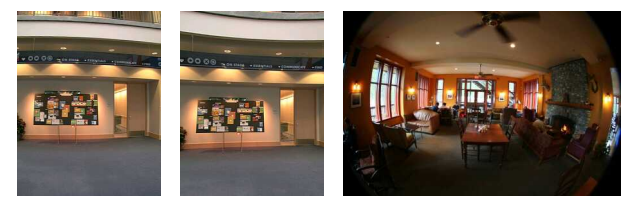
\includegraphics[width=.9\linewidth]{figures/c2/radial_distortion.png}
       \caption[Các loại biến dạng xuyên tâm]{Các loại biến dạng xuyên tâm: (a) barrel, (b) pincushion, và (c) mắt cá. Hình ảnh mắt cá kéo dài gần 180° từ bên này sang bên kia \cite{Szeliski22Book}.}
       \label{fig:radial_distortion}
   \end{center}
\end{figure}

\subsubsection{Biến dạng tiếp tuyến}

Biến dạng tiếp tuyến xảy ra do ống kính và cảm biến ảnh không được căn chỉnh song song hoàn hảo. Nó thường được mô hình hóa bằng hai hệ số $p_1$ và $p_2$. Tọa độ pixel bị biến dạng $(u_d, v_d)$ do biến dạng tiếp tuyến có thể được tính như sau:

\begin{equation}
    \begin{aligned}
x_d &= x + [2 p_1 xy + p_2 (r^2 + 2 x^2)] \\
y_d &= y + [p_1 (r^2 + 2 y^2) + 2 p_2 xy]
\end{aligned}
\end{equation}


\subsubsection{Khử biến dạng}

Mục tiêu của việc khử biến dạng là tìm lại tọa độ pixel không bị biến dạng $(u, v)$ từ tọa độ pixel bị biến dạng $(u_d, v_d)$ và các hệ số biến dạng. Quá trình này thường phức tạp hơn vì các phương trình biến dạng là phi tuyến. Một số phương pháp khử biến dạng bao gồm : 

\begin{itemize}
\item Phương pháp trực tiếp: Cố gắng giải trực tiếp hệ phương trình biến dạng để tìm $(u, v)$ từ $(u_d, v_d)$.
\item Phương pháp lặp: Sử dụng các thuật toán lặp để tìm ra giá trị $(u, v)$ sao cho khi áp dụng mô hình biến dạng, ta thu được giá trị gần đúng với $(u_d, v_d)$ nhất.
\item Sử dụng bản đồ ánh xạ: Tính toán một bản đồ ánh xạ từ tọa độ pixel bị biến dạng sang tọa độ pixel không bị biến dạng và sau đó áp dụng bản đồ này lên ảnh. Đây cũng là cách thư viện OpenCV sử dụng để khử biến dạng bằng việc cung cấp các hàm cv2.undistort và cv2.remap.
\end{itemize}

\section{Phép đạc tam giác}

Phép đạc tam giác (hay triangulation) là một kỹ thuật cơ bản trong thị giác máy tính và tái tạo 3D, được sử dụng để xác định vị trí 3D của một điểm trong không gian dựa trên hình chiếu của nó trên hai hoặc nhiều ảnh được chụp từ các vị trí máy ảnh khác nhau với các tham số máy ảnh đã biết. 

Nguyên lý của phép đạc tam giác dựa trên việc mỗi điểm ảnh trên một bức ảnh tương ứng với một tia sáng trong không gian 3D, xuất phát từ tâm máy ảnh và đi qua điểm ảnh đó. Nếu chúng ta có hai hoặc nhiều ảnh của cùng một điểm 3D, mỗi ảnh sẽ tạo ra một tia sáng tương ứng. Vị trí 3D của điểm đó là giao điểm của các tia sáng này. 

Giả sử chúng ta có hai máy ảnh với ma trận chiếu $\mathbf{P}_1$ và $\mathbf{P}_2$. Một điểm 3D $\mathbf{X} = [X, Y, Z, 1]^T$ được chiếu lên ảnh 1 tại điểm $\mathbf{x}_1 = [u_1, v_1, 1]^T$ và lên ảnh 2 tại điểm $\mathbf{x}_2 = [u_2, v_2, 1]^T$. Theo mô hình máy ảnh pinhole, ta có:


\begin{equation} \label{eq:your_label_here} % Thêm label nếu cần tham chiếu
\begin{aligned}
    s_1 \mathbf{x}_1 &\sim \mathbf{P}_1 \mathbf{X} \\
    s_2 \mathbf{x}_2 &\sim \mathbf{P}_2 \mathbf{X}
\end{aligned}
\end{equation}


Trong đó $s_1$ và $s_2$ là các hệ số tỷ lệ (thường liên quan đến độ sâu của điểm), và $\sim$ biểu thị đẳng thức theo tỷ lệ.

Để tìm $\mathbf{X}$, chúng ta có thể viết lại các phương trình trên thành hệ thống các phương trình tuyến tính. Từ $\mathbf{x}_1 \times (\mathbf{P}_1 \mathbf{X}) = \mathbf{0}$ và $\mathbf{x}_2 \times (\mathbf{P}_2 \mathbf{X}) = \mathbf{0}$, ta thu được một hệ thống các phương trình tuyến tính đồng nhất với ẩn số (X, Y, Z, 1). Chúng ta có thể giải hệ thống này bằng các phương pháp như phân tích giá trị suy biến (hay Singular Value Decomposition - SVD) để tìm ra nghiệm $\mathbf{X}$.   

